\documentclass[pdf]{beamer}
\ProvidesPackage{preamble_slides}

% %% Beamer Stuff
\usetheme{Berlin}
\setbeamertemplate{footline}[frame number]
\setbeamertemplate{caption}[numbered]
\setbeamertemplate{section in toc}[sections numbered]
\setbeamertemplate{subsection in toc}[sections numbered]
\setbeamertemplate{navigation symbols}{} 
\setbeamercovered{transparent=25}
\usepackage{graphicx}
\usepackage{hhline}
\usepackage{appendixnumberbeamer}
\usepackage{multirow}
\definecolor{maincolor}{rgb}{0.6, 0.4, 0.7}
\usecolortheme[named = maincolor]{structure}
\renewcommand{\arraystretch}{1.5}

%% Bibliography packages
\usepackage{natbib}
\bibliographystyle{abbrvnat}

\title{Chinese Head Tax Project: Updates}
\author{Amy Kim}
\date{July 21, 2023}

\begin{document}
\begin{frame}[plain]
    \titlepage
\end{frame}

\begin{frame}{Research Question}
    How does an increase in fixed migration costs (in the form of a nationality-specific flat `head tax' at the time of entry) affect selection into immigration?
\end{frame}


% \begin{frame}{Paper Outline & Updates}
% \begin{itemize}
%     \item Intro, Background, Data
%     \item Effects on Immigration Inflow -- \textit{Updated} key figure & regressions 
%     \item Effects on Outcomes -- \textit{Redid} key figure & regressions 
%     \item Comparison with US -- \textit{Added} new figure, 
% \end{itemize}
% \end{frame}

% PART 1: IMMIGRATION INFLOW EFFECTS
\section{Immigration Inflow}
\begin{frame}[label = fig2_flow]
    \frametitle{Immigration Inflow: Updated Figure}
    \centering 
    \begin{figure}
        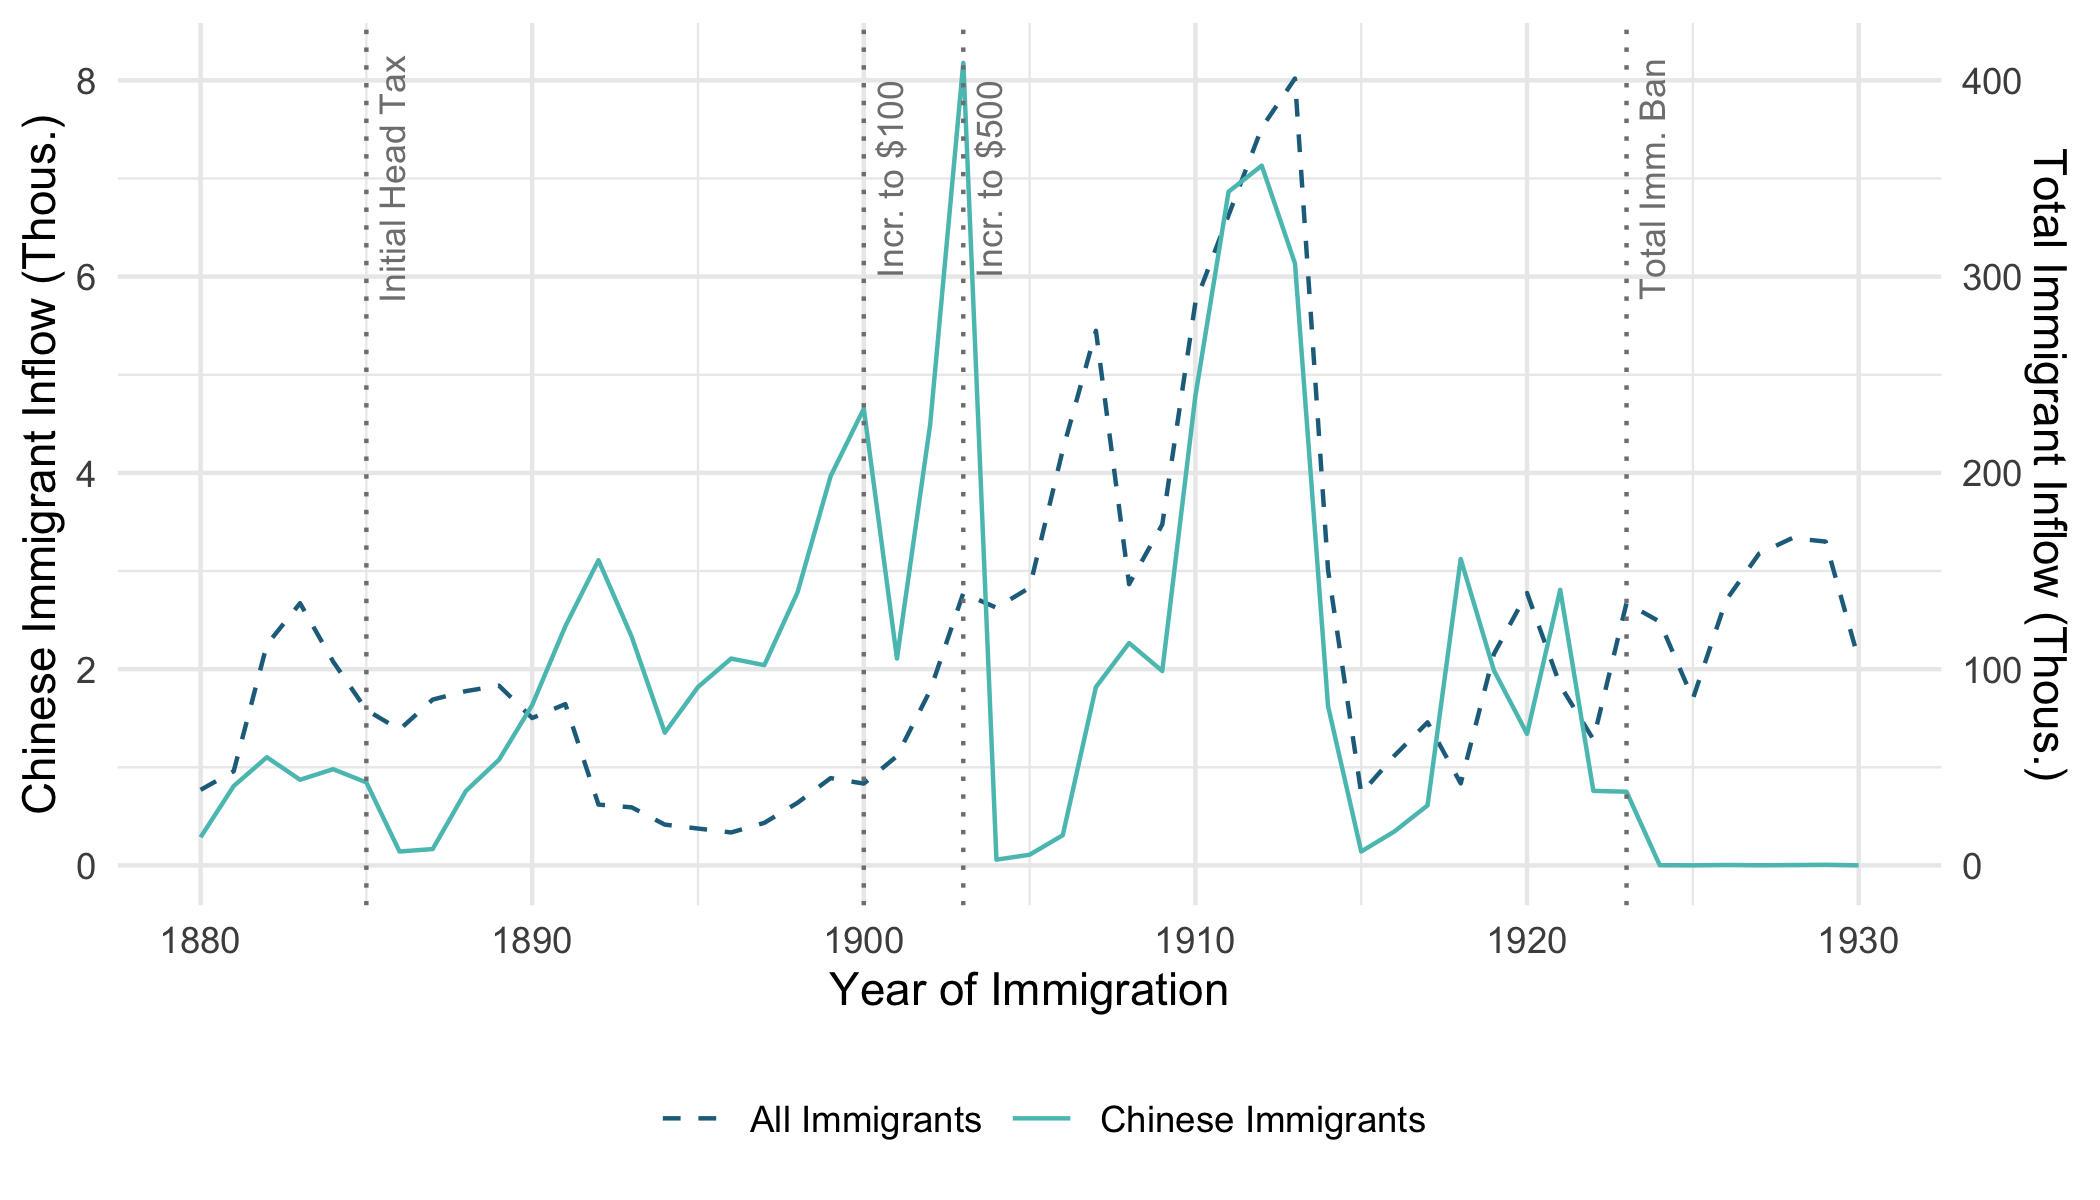
\includegraphics[width = \textwidth]{../../figs/fig2_flow.png}
    \end{figure}
    \hyperlink{fig2_flow_old}{\beamerbutton{Previous Version}}
\end{frame}

\begin{frame}[label = flow_reg]
    \frametitle{Immigration Inflow: Regression Specification}
    \begin{equation*}
        \text{CHIFLOW}_t = \alpha + x_t' \beta + \delta_1 t + \delta_2 t^2 + \sum_{\tau \in \mathcal{T}} \gamma_\tau \mathbf{1}[TAX_t = \tau] 
    \end{equation*}
    \begin{itemize}
        \item $TAX_t$ is tax paid in year $t$ (\$50 tax is omitted for Register; \$0 tax is omitted for Census)
        \item $x_t$ includes total immigration inflow + economic condition (GNP growth)
        \item (quadratic) time trend seems necessary \hyperlink{flow_diff}{\beamerbutton{Normalized Chinese Inflow}} but complicates coeff interpretation -- exclude constant?
        \item Count years of change as lower head tax (e.g. categorize 1885 as \$0 head tax since established in July 1885)
        \item Dissipation of effect within a few years?
        \item Standardize variables?
    \end{itemize}
\end{frame}

\begin{frame}[label = tab2_flow]
    \frametitle{Immigration Inflow: Regression Results}
    \centering
    \begin{table}[H]
		\resizebox{\textwidth}{!}{
            
% Table created by stargazer v.5.2.3 by Marek Hlavac, Social Policy Institute. E-mail: marek.hlavac at gmail.com
% Date and time: Mon, Jul 17, 2023 - 15:10:09
\begin{tabular}{@{\extracolsep{5pt}}lccccc} 
\\[-1.8ex]\hline 
\hline \\[-1.8ex] 
 & \multicolumn{5}{c}{\textit{Dependent variable:}} \\ 
\cline{2-6} 
\\[-1.8ex] & $CHIFLOW^R$ (Register) & $CHIFLOW^C$ (Census) & $JAPANFLOW^C$ (Census) & $CHIFLOW^C$ (Pre-1908) & $JAPANFLOW^C$ (Pre-1908) \\ 
\\[-1.8ex] & (1) & (2) & (3) & (4) & (5)\\ 
\hline \\[-1.8ex] 
 \$50 Tax &  & $-$453.700 & $-$383.200 & $-$96.840 & $-$56.450 \\ 
  &  & (399.800) & (242.300) & (294.200) & (187.600) \\ 
  & & & & & \\ 
 \$100 Tax & $-$695.100 & $-$599.000 & $-$867.000$^{**}$ & $-$283.200 & $-$1,089.000$^{***}$ \\ 
  & (834.500) & (604.800) & (366.500) & (353.100) & (225.100) \\ 
  & & & & & \\ 
 \$500 Tax & $-$6,989.000$^{***}$ & $-$1,607.000$^{**}$ & $-$810.100$^{*}$ & $-$1,188.000$^{**}$ & $-$1,620.000$^{***}$ \\ 
  & (1,006.000) & (669.300) & (405.600) & (471.200) & (300.500) \\ 
  & & & & & \\ 
\hline \\[-1.8ex] 
Observations & 38 & 41 & 41 & 28 & 28 \\ 
Adjusted R$^{2}$ & 0.747 & 0.675 & 0.430 & 0.730 & 0.833 \\ 
\hline 
\hline \\[-1.8ex] 
\textit{Note:}  & \multicolumn{5}{r}{$^{*}$p$<$0.1; $^{**}$p$<$0.05; $^{***}$p$<$0.01} \\ 
\end{tabular} 

		}
	\end{table}  
    \hyperlink{census_flow}{\beamerbutton{Census Inflow w/ Japanese Imm.}}
\end{frame}

%%%%%%%%%%%%%%%%%%%%%%%%%%%%%%%%%%%%%%%%%%%%%%%%%%%%%%%
%%%%%%%%%%      A  P  P  E  N  D  I  X      %%%%%%%%%%%
%%%%%%%%%%%%%%%%%%%%%%%%%%%%%%%%%%%%%%%%%%%%%%%%%%%%%%%
\appendix

%---------------------------
%  Short Paper Version of Immigration Inflow Graph
%---------------------------

\begin{frame}[label = fig2_flow_old]
	\frametitle{Immigration Inflow: Old Figure}
    \centering
	\begin{figure}[H]
		\begin{center}
			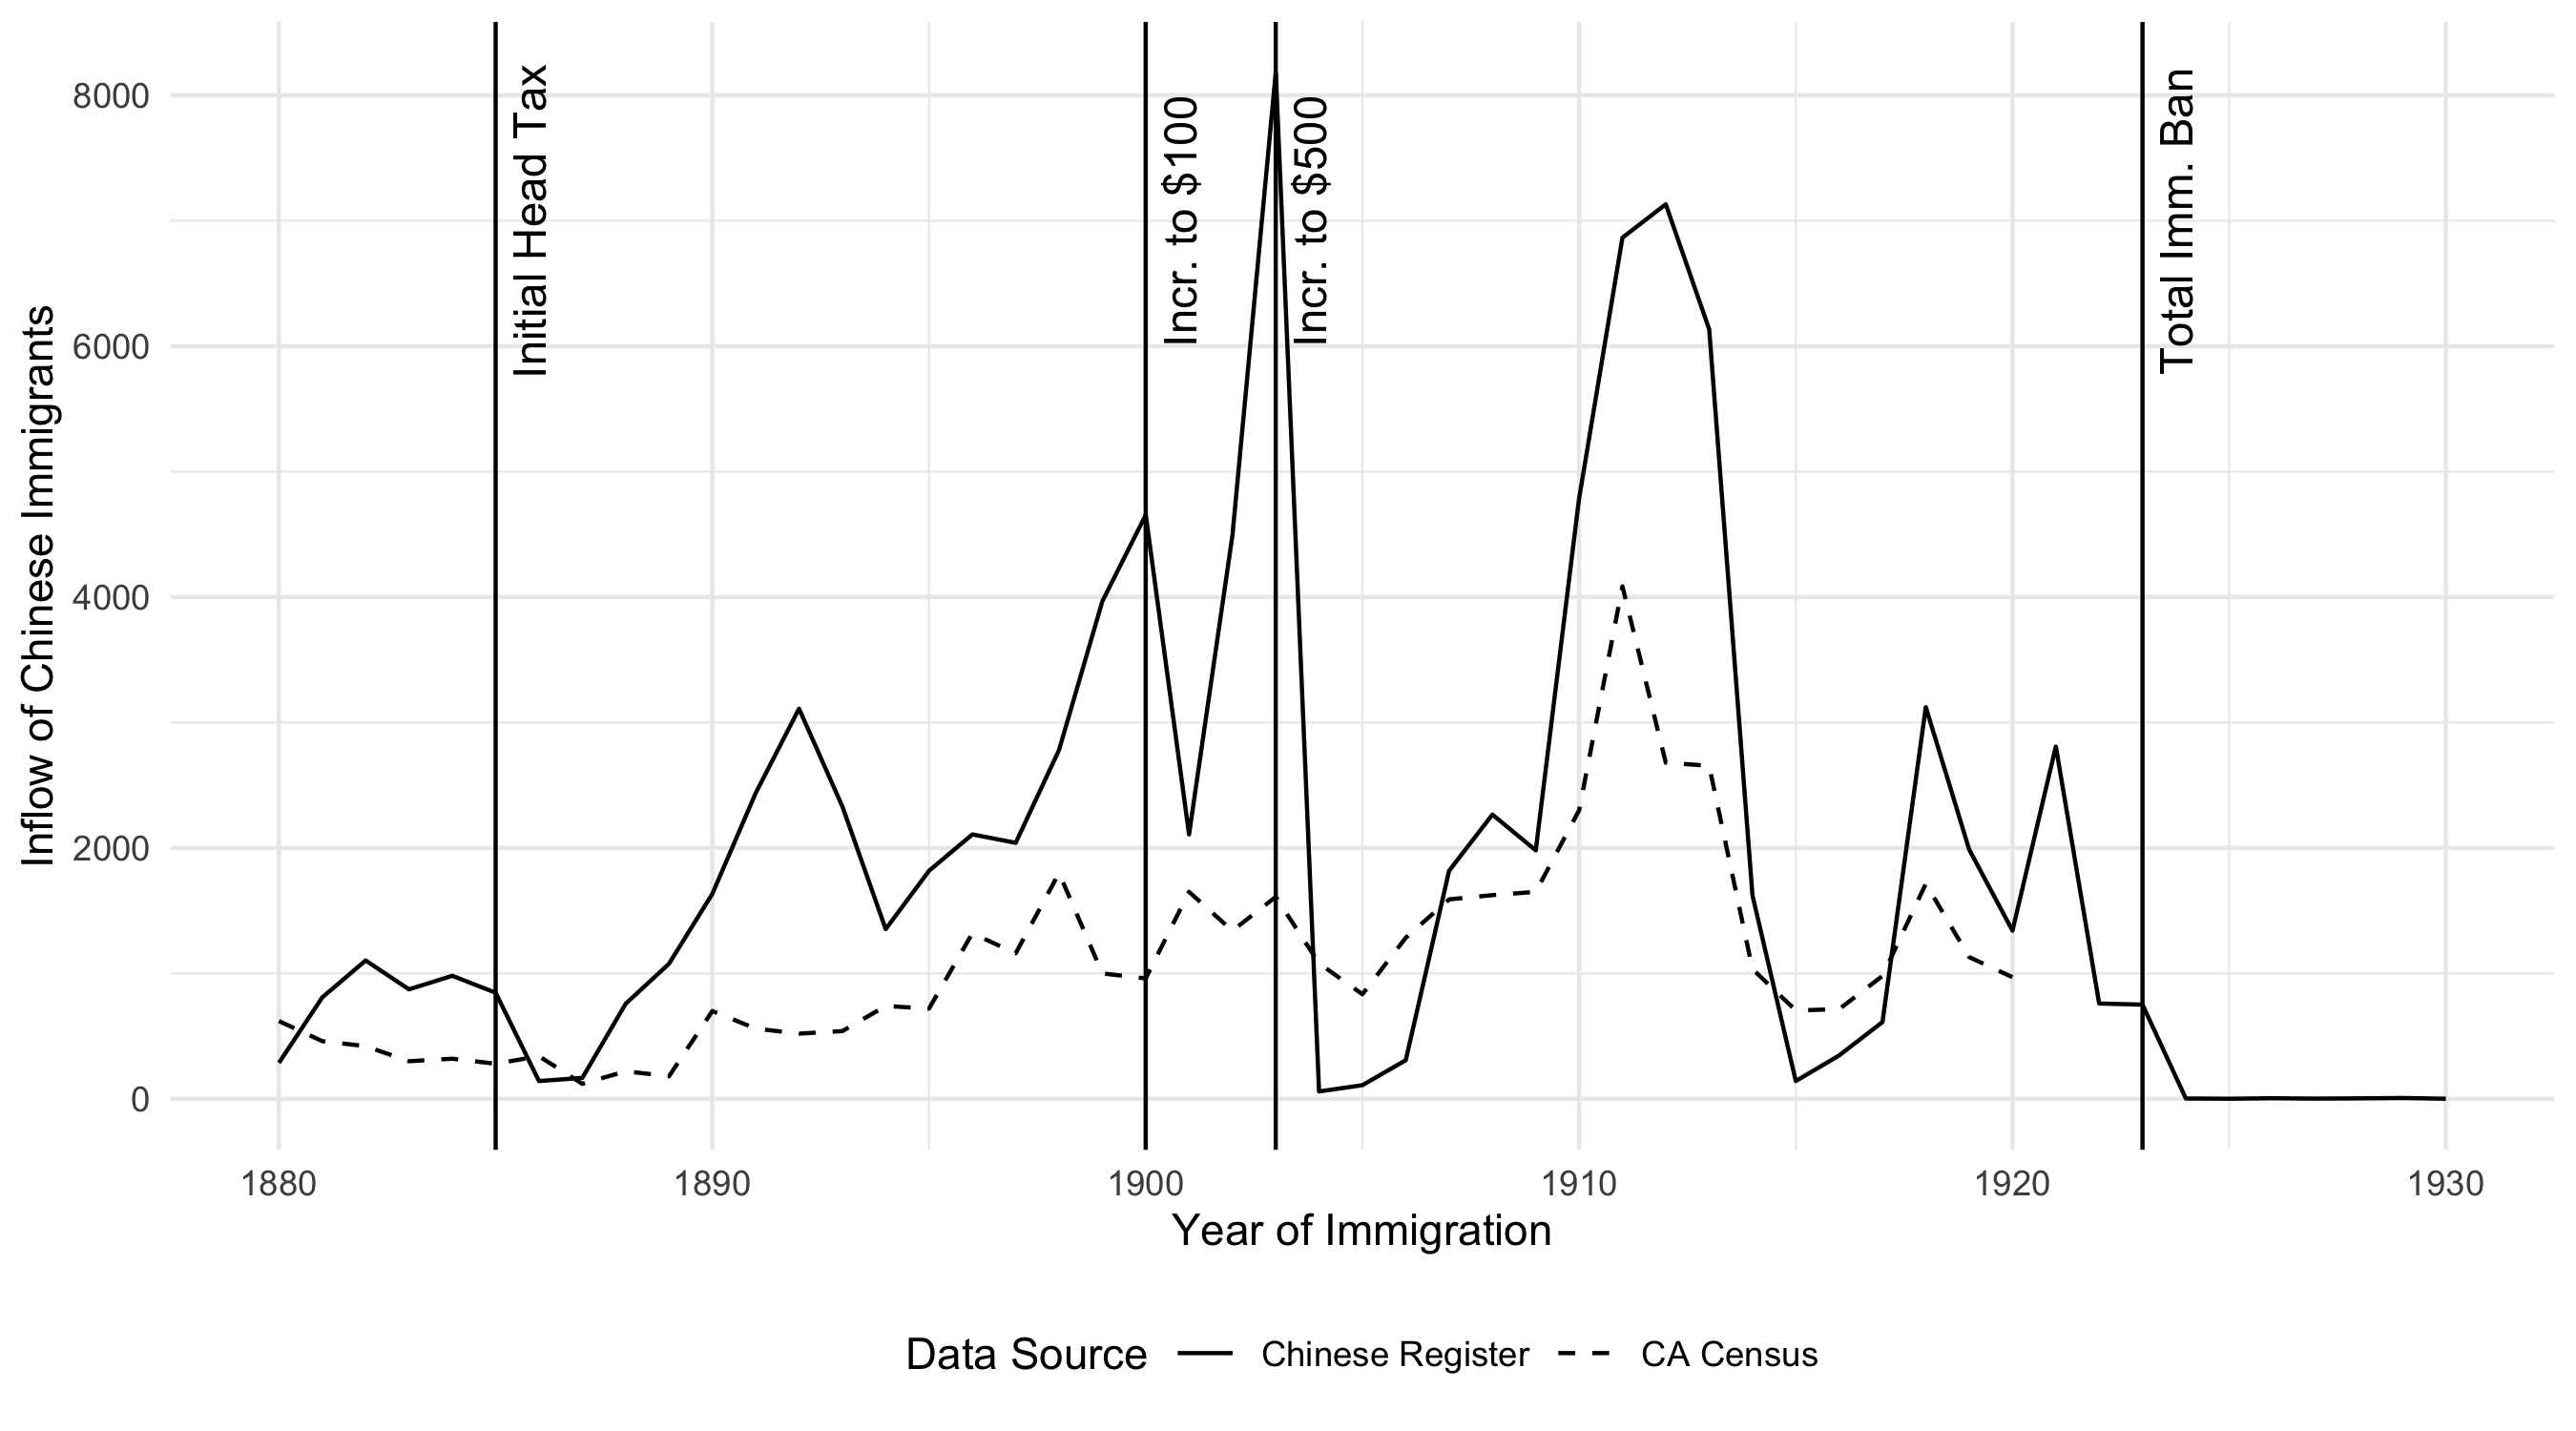
\includegraphics[width=\textwidth]{../../figs/shortpaper_figs/fig2_flow.png}
		\end{center}
	\end{figure}
    \hyperlink{fig2_flow}{\beamerbutton{Back to Slides}}
\end{frame}

%---------------------------
%  Normalized Chinese Inflow (Inflow Diff)
%---------------------------

\begin{frame}[label = flow_diff]
	\frametitle{Chinese Immigration Inflow as Fraction of Total}
    \centering
	\begin{figure}[H]
		\begin{center}
			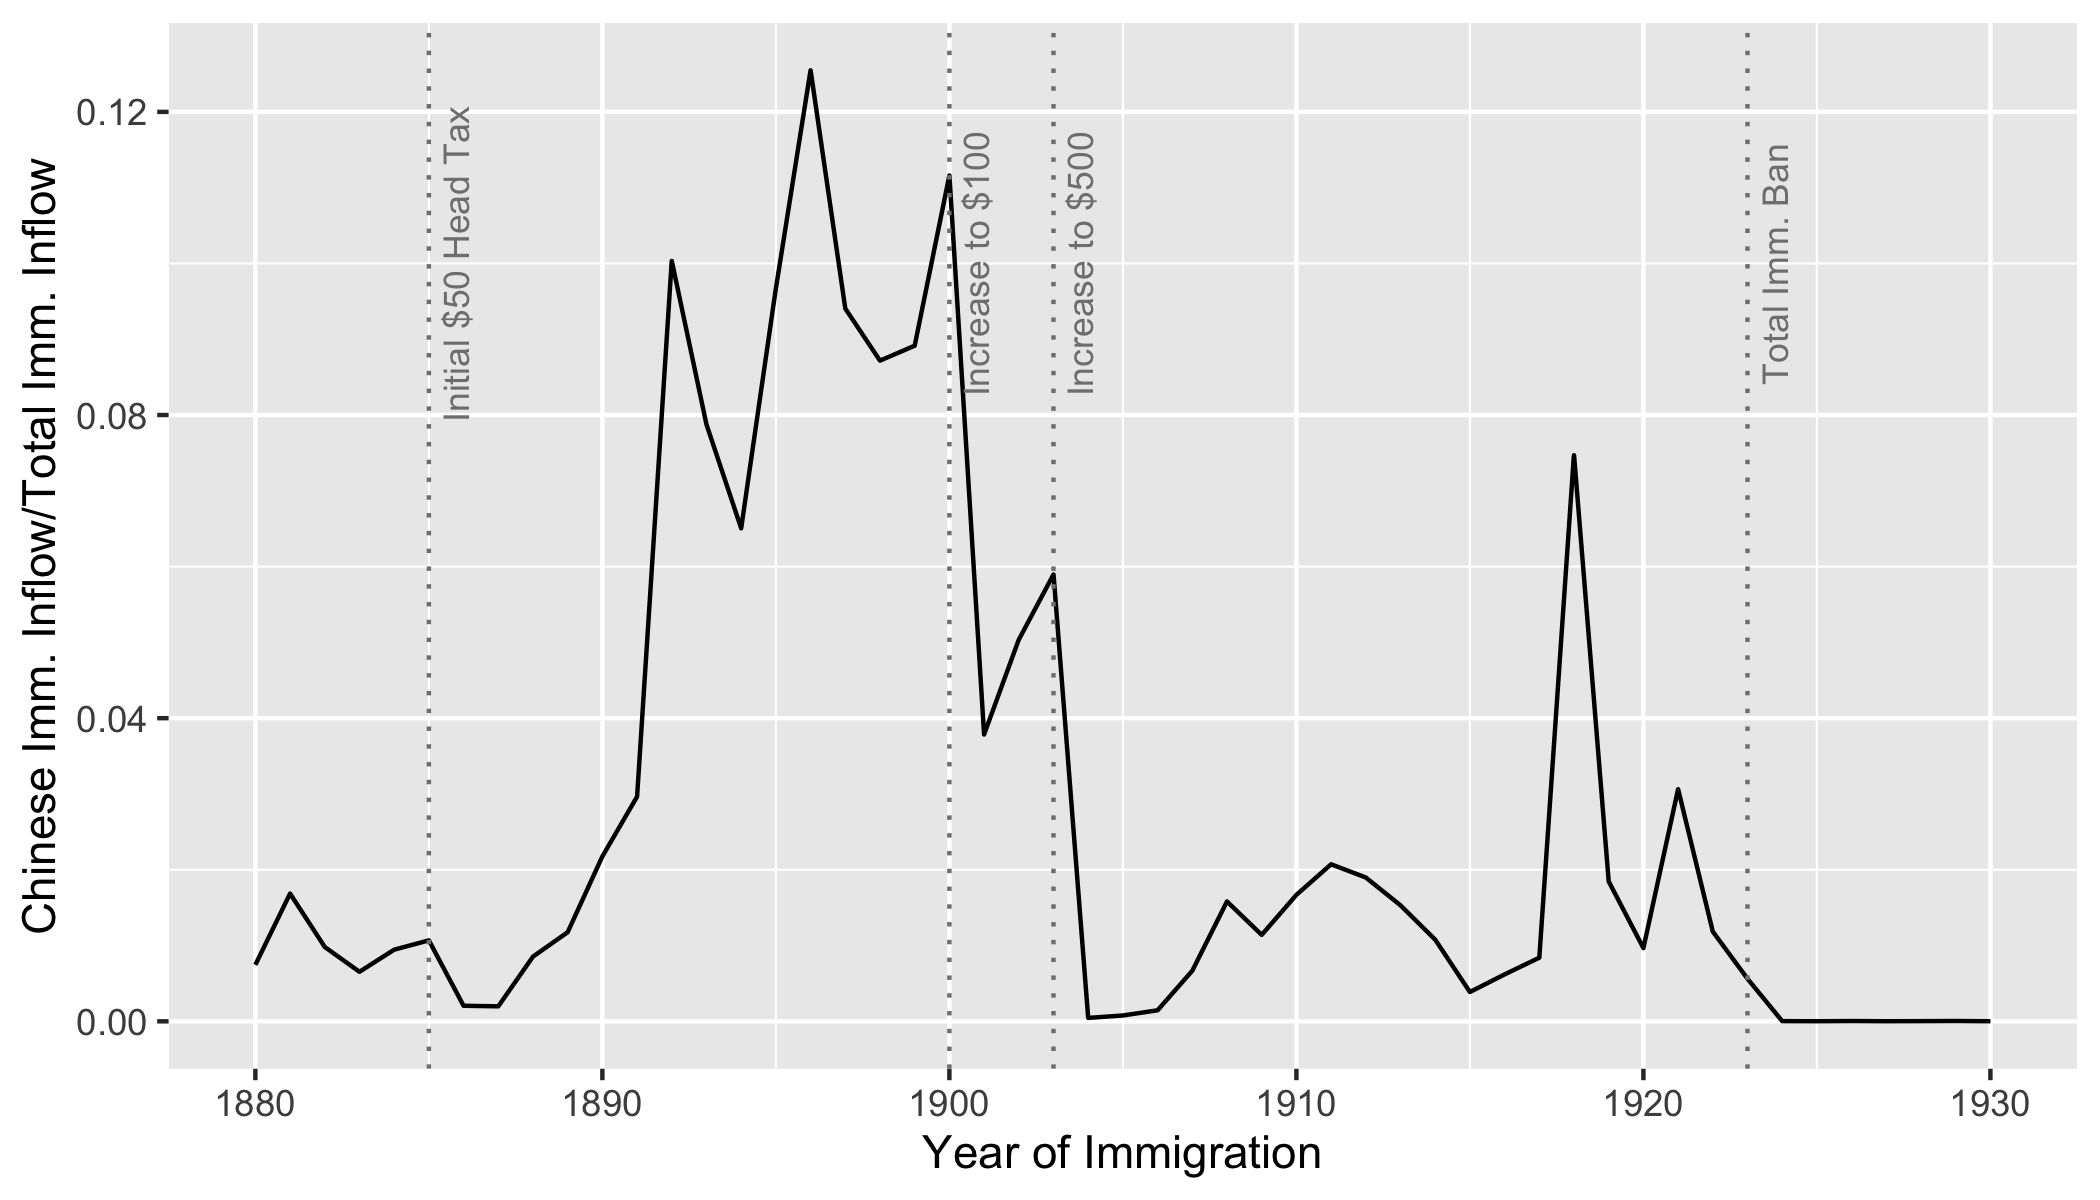
\includegraphics[width=\textwidth]{../../figs/21jul23/flowpct.png}
		\end{center}
	\end{figure}
    \hyperlink{flow_reg}{\beamerbutton{Back to Slides}}
\end{frame}

%---------------------------
%  Census Inflow w/ Japanese
%---------------------------

\begin{frame}[label = census_flow]
	\frametitle{Immigration Inflow with Census Data}
    \centering
	\begin{figure}[H]
		\begin{center}
			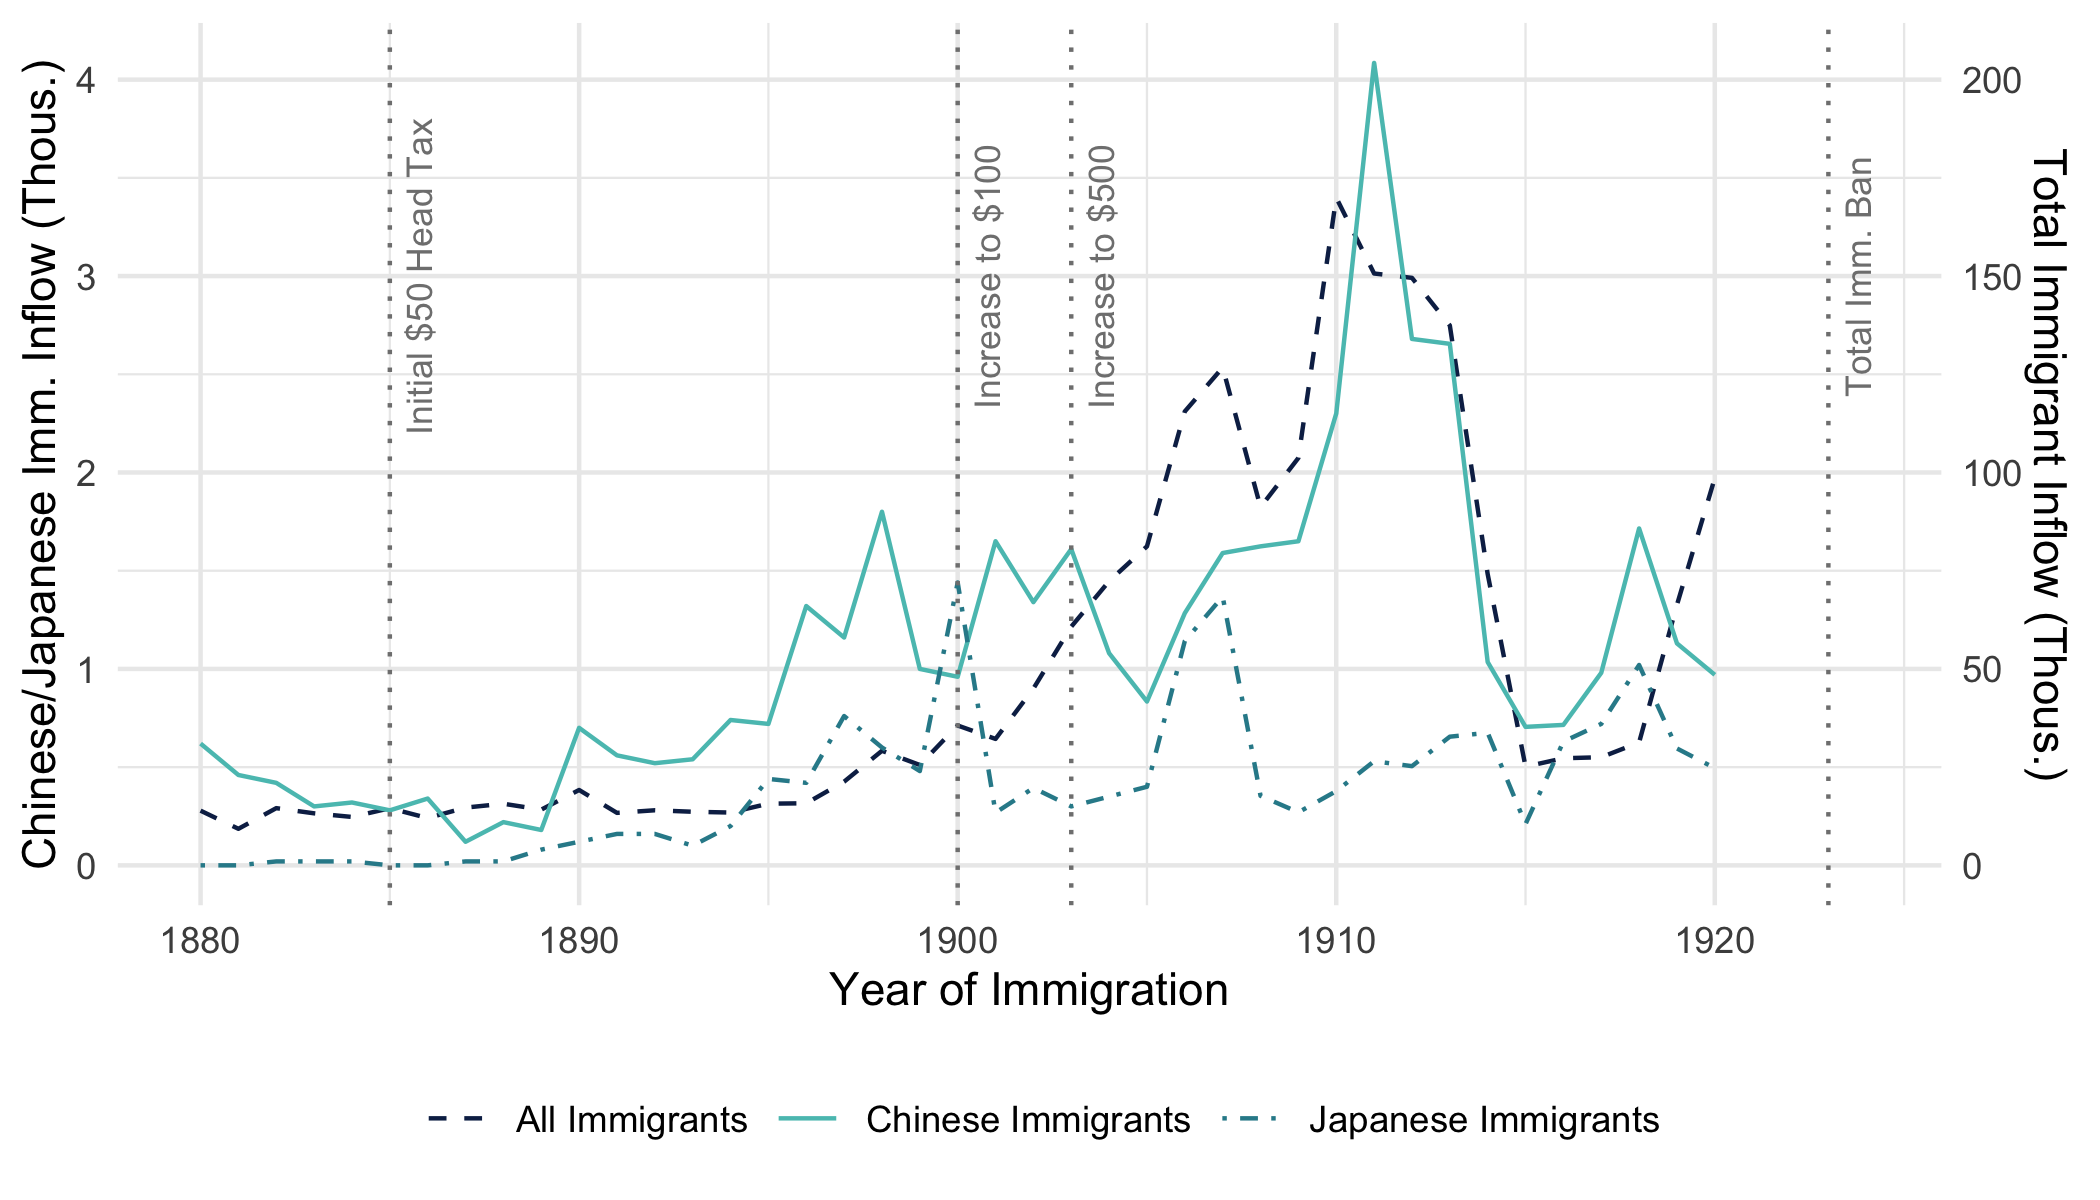
\includegraphics[width=\textwidth]{../../figs/21jul23/fig2_flow_jap.png}
		\end{center}
	\end{figure}
    \hyperlink{tab2_flow}{\beamerbutton{Back to Slides}}
\end{frame}

% %---------------------------
% %   Density of Chinese Immigration to Canada by Date
% %---------------------------

% \begin{frame}[label = dateimmchi]
% 	\frametitle{Chinese Immigration to Canada Using Cross-Year Means for Census Data}
%     \centering
% 	\begin{figure}[H]
% 		\begin{center}
% 			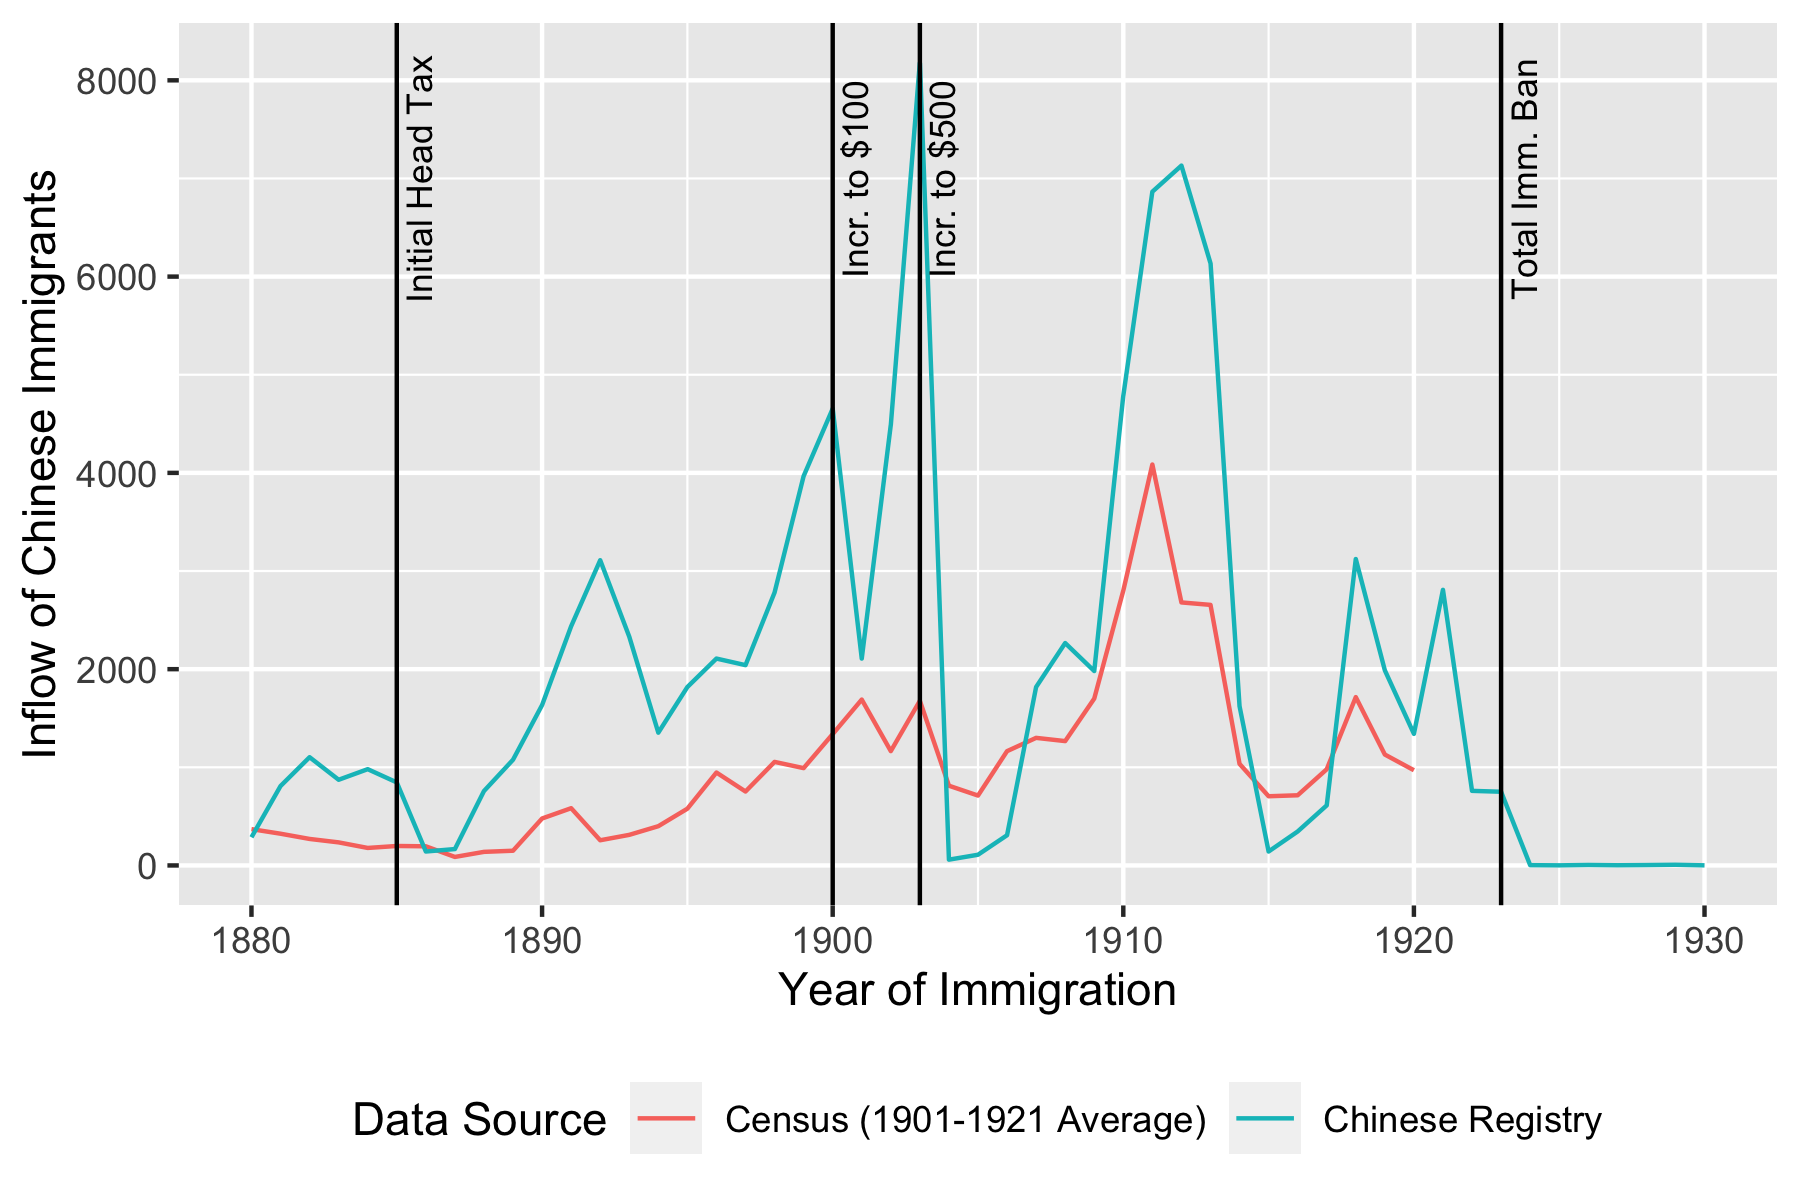
\includegraphics[width=0.9\textwidth]{../../figs/yrimmchi_means.png}
% 		\end{center}
% 	\end{figure}
%     \hyperlink{yrimmchi}{\beamerbutton{Back to Slides}}
% \end{frame}

% %---------------------------
% %   Major Events in 1910s
% %---------------------------
% \begin{frame}[label = events1912]
% 	\frametitle{Relevant Events in the 1910s}
% 	\begin{itemize}
%         \item Canada [1910]: Immigration Act of 1910 further restricts immigration, not expands
%         \item Canada [1912]: Head Tax Certificates reissued with photo 
%         \begin{itemize}
%             \item Unlikely to have such a massive spike just from using other people's certificates 
%         \end{itemize}
%         \item China: Republic of China established in 1912 following Xinhai Revolution (1911)
%         \begin{itemize}
%             \item If this is primary cause of spike, would expect some change in regional origin of Chinese immigrants \hyperlink{originchi}{\beamerbutton{Chinese Immigration by Origin by Year}}
%             \item Also would not expect to see spike in immigration from other countries \hyperlink{yrimmall}{\beamerbutton{Immigration to Canada from Different Countries}}
%         \end{itemize}
%         \item Worldwide: WWI begins July 1914
%         \begin{itemize}
%             \item Unclear why most of spike is prior to 1914 -- general global unrest?
%         \end{itemize}
%     \end{itemize}
%     \hyperlink{yrimmchi}{\beamerbutton{Back to Slides}}
% \end{frame}

% %---------------------------
% %   Chinese immigration by Origin County
% %---------------------------
% \begin{frame}[label = originchi]
% 	\frametitle{Chinese Immigration by County of Origin in China}
%     \centering
% 	\begin{figure}[H]
% 		\begin{center}
% 			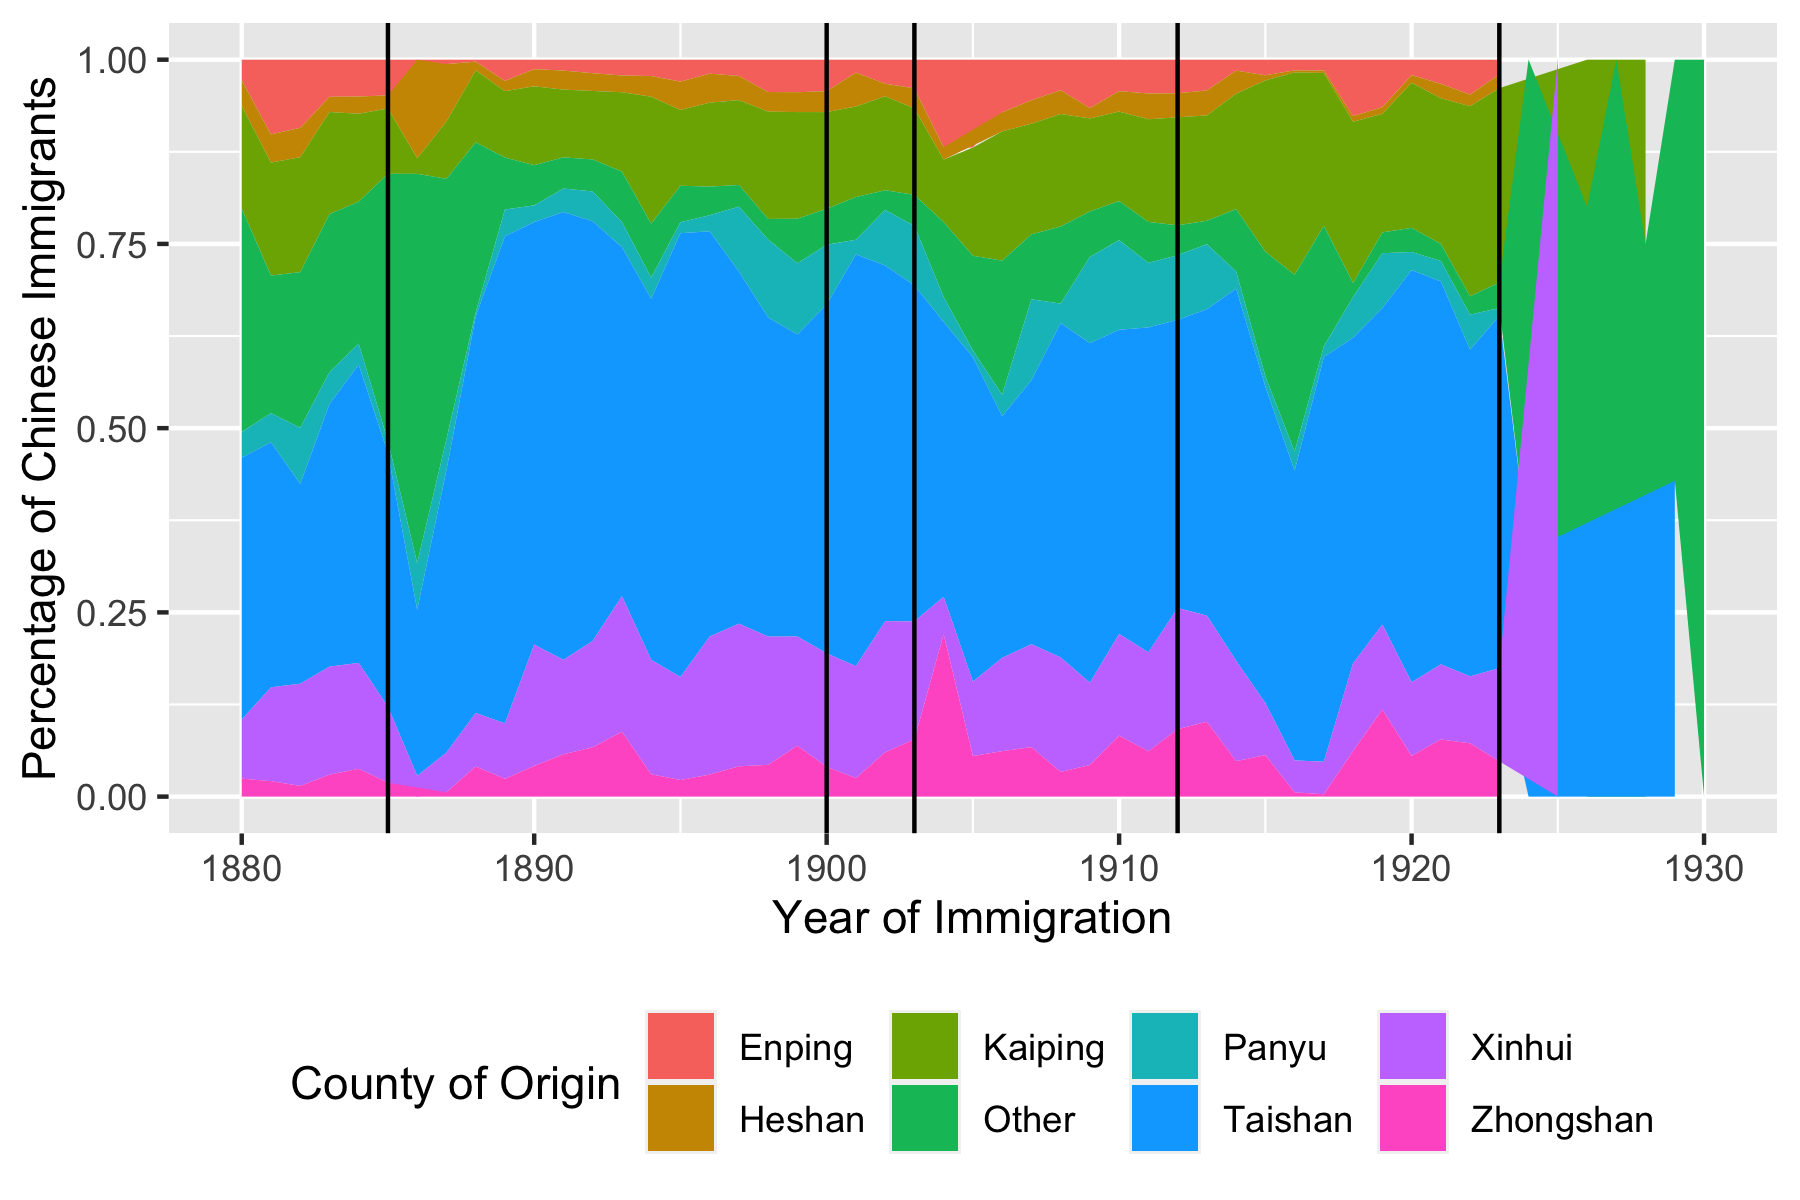
\includegraphics[width=0.9\textwidth]{../../figs/chiorig.png}
% 		\end{center}
% 	\end{figure}
%     \hyperlink{events1912}{\beamerbutton{Back to 1910s Events}}
% \end{frame}

\end{document}